\documentclass[11pt,letterpaper]{article}
\usepackage[margin=1in,headheight=14pt]{geometry}
\usepackage[T1]{fontenc}
\usepackage{lmodern}
\usepackage{amsmath,amssymb,amsthm,mathtools}
\usepackage{graphicx,booktabs,array,longtable}
\usepackage{xcolor,microtype,enumitem}
\usepackage{fancyhdr}
\usepackage{placeins}
\usepackage{xurl}
\usepackage[colorlinks=true,linkcolor=teal!60!black,citecolor=teal!60!black,urlcolor=teal!60!black]{hyperref}
\usepackage[nameinlink,noabbrev]{cleveref}
\usepackage{listings}
\definecolor{ink}{HTML}{18364A}
\definecolor{teal}{HTML}{087E8B}
\definecolor{pale}{HTML}{EDF5F7}
\hypersetup{pdftitle={Constructive Stokes in Intuitionistic Primitive Recursive Arithmetic},
  pdfauthor={Research report prepared for Vladimir Reshetnikov},
  pdfsubject={Quantitative cubical Stokes, effective analysis, and iPRA formalization}}
\pagestyle{fancy}
\fancyhf{}
\fancyhead[L]{\small\color{ink}Constructive Stokes in iPRA}
\fancyhead[R]{\small November 2026}
\fancyfoot[C]{\thepage}
\setlength{\parskip}{0.35em}
\setlength{\parindent}{1.1em}
\setlength{\emergencystretch}{2em}
\renewcommand{\topfraction}{0.88}
\renewcommand{\textfraction}{0.10}
\setlist{topsep=0.25em,itemsep=0.2em}
\setcounter{tocdepth}{1}
\lstset{basicstyle=\ttfamily\footnotesize,breaklines=true,columns=fullflexible,
  frame=single,rulecolor=\color{black!20},backgroundcolor=\color{black!2},
  showstringspaces=false}
\newtheorem{theorem}{Theorem}[section]
\newtheorem{lemma}[theorem]{Lemma}
\newtheorem{proposition}[theorem]{Proposition}
\newtheorem{corollary}[theorem]{Corollary}
\theoremstyle{definition}
\newtheorem{definition}[theorem]{Definition}
\newtheorem{example}[theorem]{Example}
\theoremstyle{remark}
\newtheorem{remark}[theorem]{Remark}
\newcommand{\N}{\mathbb N}
\newcommand{\Z}{\mathbb Z}
\newcommand{\Q}{\mathbb Q}
\newcommand{\R}{\mathbb R}
\newcommand{\ipra}{\mathsf{iPRA}}
\newcommand{\PR}{\mathsf{PR}}
\newcommand{\eps}[1]{2^{-#1}}
\newcommand{\abs}[1]{\left|#1\right|}
\newcommand{\norm}[1]{\left\|#1\right\|_\infty}
\newcommand{\cube}[1]{[0,1]^{#1}}
\newcommand{\Grid}[2]{\{0,\ldots,#1-1\}^{#2}}
\newcommand{\dd}{\mathrm d}
\newcommand{\clog}[1]{\left\lceil\log_2\max\{1,#1\}\right\rceil}
\newcommand{\EqName}{\mathrel{\simeq}}
\newcommand{\RepoCommit}{\texttt{a5688a1b37d62046c894691c3c41f7bdd53976ca}}
\DeclareMathOperator{\curl}{curl}
\DeclareMathOperator{\diver}{div}
\DeclareMathOperator{\clip}{clip}
\DeclareMathOperator{\sgn}{sgn}
\begin{document}
\begin{titlepage}
\vspace*{0.8in}
{\large\color{teal}\sffamily CONSTRUCTIVE ANALYSIS / PROOF THEORY\par}
\vspace{0.45in}
{\Huge\bfseries\color{ink}Constructive Stokes\par}
\vspace{0.15in}
{\LARGE\color{ink}in intuitionistic primitive\\recursive arithmetic\par}
\vspace{0.4in}
{\large A finite cubical proof, explicit precision bounds,\\
curved parameterizations, and a Lean formalization plan\par}
\vspace{0.55in}
{\large Prepared for Vladimir Reshetnikov\par}
{\large November 21, 2026\par}
\vfill
\noindent\colorbox{pale}{\parbox{\dimexpr\textwidth-2\fboxsep\relax}{
\textbf{Main result.} For supplied primitive recursive coefficient names,
uniform continuity certificates, and uniform first-order remainder certificates,
Stokes' identity is provable as a schema in first-order $\ipra$.
The proof constructs both integrals and an explicit rate witnessing their equality.
It extends to finite chains of certified $C^2$ parameterizations.
}}
\vspace{0.3in}
\noindent\textbf{Verification status.}
The mathematical proof and arithmetic reduction are developed in this report.
The accompanying Lean files are a formalization outline with proof scripts;
they have not been compiled in this environment. No completed Lean proof of
the full Stokes theorem is claimed. Exact-arithmetic Python checks exercise
the finite identities and the worked example.
\end{titlepage}

\begin{abstract}
We prove a constructive Stokes theorem for finite, explicitly presented
parameterized cubical chains. The analytic input consists of primitive recursive
rational evaluations with supplied uniform moduli and first-order remainder
certificates. On a $k$-cube, an exact telescoping identity gives the rational bound
\[
 \abs{V_{n,p}-B_{n,p}}
 \le k\,2^{-t}+k(2^{n+1}+1)2^{-p}
 \qquad(n\ge\tau(t)).
\]
Here $V_{n,p}$ is a volume Riemann sum for the exterior derivative and $B_{n,p}$
is the oriented boundary sum. A specified primitive recursive schedule makes
both sequences regular Cauchy names and proves their equality with a rate.
Every induction in the analytic core is on a finite rational identity or
inequality, hence reduces to quantifier-free induction.

We develop the named-real and integration conventions, prove effective product
and composition rules without assuming an integral theorem, establish
$\dd(\sigma^*\omega)=\sigma^*(\dd\omega)$ by finite alternating algebra, and
deduce Kelvin--Stokes, Green, and divergence identities for supplied cell
presentations. A curved polynomial example is worked out exactly. The
formalization plan identifies concrete object-level iPRA lemmas already in
ProveIt, and separates them from the remaining signed-rational, multidimensional,
and geometric obligations.
\end{abstract}
\tableofcontents
\newpage
\section{The theorem and the precise constructive scope}\label{sec:scope}

The familiar Kelvin--Stokes formula is
\begin{equation}\label{eq:kelvin-intro}
 \int_{\partial S}\mathbf F\cdot\dd\mathbf r
 =\int_S(\curl\mathbf F)\cdot\mathbf n\,\dd S.
\end{equation}
The differential-form version is
\begin{equation}\label{eq:stokes-intro}
 \int_{\partial C}\omega=\int_C\dd\omega.
\end{equation}
These are the classical target identities; see the source supplied in the
request and the primary expositions in \cite{dyatlov,poonen}. Our contribution
here is an explicit arithmetic proof for effective input presentations. No
claim of novelty for the classical telescoping argument is intended.

There are two separate questions. First, can a domain, a coefficient function,
and an integral be represented using primitive recursive data? Second, can the
identity between the resulting quantities be proved using only the induction
available in $\ipra$? A statement in ordinary Lean about $\R$, or even about
computable reals, does not by itself answer the second question.

\subsection{What the input must contain}

A basic $k$-dimensional cell is the parameter cube $Q^k=\cube{k}$, $k\ge1$.
Its coefficients are given by fixed primitive recursive programs
\[
 F_i(x,p),\ G_i(x,p)\in\Q \qquad(1\le i\le k,\ x\in Q^k\cap\Q^k,\ p\in\N).
\]
The intended interpretation is that $F_i(x,p)$ approximates $f_i(x)$ and
$G_i(x,p)$ approximates $\partial_i f_i(x)$ to error at most $2^{-p}$.
The theorem does not merely assume that these interpretations are plausible.
It requires the explicit arithmetic coherence, continuity, and remainder
conditions in \cref{sec:certificates}. The moduli in those conditions are
themselves fixed primitive recursive functions.

For a curved cell in an ambient rational box, the input additionally provides
a primitive recursive $C^2$ parameterization $\sigma:Q^k\to\R^m$ with certified
first and second jets, bounds, and uniform moduli. An ambient $(k-1)$-form
has certified $C^1$ coefficients. All occurrences of real-valued functions in
this description are shorthand for rational approximation programs and the
specified arithmetic certificates.

A finite chain is a supplied list
\[
 C=\sum_{\lambda<L}c_\lambda\sigma_\lambda,\qquad c_\lambda\in\Z.
\]
Its boundary is computed from the faces of that list. If interior faces are
to be identified, their matching data are supplied explicitly. The proof
does not search for a cubulation, decide equality of arbitrary functions,
or extract a uniform modulus from a bare continuity assertion.

\begin{theorem}[Constructive Stokes, informal form]\label{thm:informal}
For each fixed collection of primitive recursive programs satisfying the
certificates specified in this report, there are primitive recursive regular
Cauchy names for $\int_C\dd\omega$ and $\int_{\partial C}\omega$.
Their equality is provable in $\ipra$ from those certificates.
For a single cube the names $V_r,B_r$ constructed below satisfy
\begin{equation}\label{eq:headline}
 \forall r\ \forall a,b\ge r,\qquad
 \abs{V_a-B_b}\le \frac{19}{64}\,2^{-r}.
\end{equation}
For a finite chain, shifting the per-cell accuracy by
$\clog{\sum_\lambda|c_\lambda|}$ gives the same stated accuracy for the chain.
\end{theorem}

The proof of the cube result is given completely in \cref{sec:finite,sec:names-proof}.
The effective calculus, pullback, and chain arguments in
\cref{sec:calculus,sec:geometry} prove the curved-cell extension.
The arithmetic interpretation in \cref{sec:ipra-audit} establishes the asserted
proof-theoretic strength.

\subsection{Why this is a substantive version of Stokes}

This result permits arbitrary fixed primitive recursive evaluation and modulus
programs satisfying the certificates, rather than only polynomial data.
The cells may be curved, multiple cells may meet along their faces, and the
result holds in every fixed finite dimension. The theorem includes the
fundamental theorem of calculus, Green's formula, ordinary surface Stokes,
and the divergence theorem for such presentations.

The restrictions concern the effective presentation and its uniformity.
It is not asserted that arbitrary classical $C^1$ data automatically possess
primitive recursive moduli. Nor is an arbitrary abstract compact manifold
automatically replaced by a supplied finite chain. An embedded surface
interpretation requires the corresponding orientation, coverage, and
compatibility data. The chain theorem itself does not require injectivity
or an immersion condition: its integrals count the supplied parameterized
cells with their multiplicities.

\subsection{The mechanism in one paragraph}

Subdivide the parameter cube into a dyadic grid. In each coordinate direction,
replace a derivative sample multiplied by the cell width by a forward
difference of coefficient samples. The remainder certificate bounds this
replacement. Sum over the entire grid. Every interior sample cancels
algebraically, leaving precisely the two opposite faces. The total error is
computed before choosing the grid. A second finite estimate compares coarse
and fine Riemann sums, thereby constructing the integrals. Finally, a
primitive recursive schedule makes both errors as small as requested.
No theorem about an unspecified limit is used as a black box.

\subsection{Relation to the repository}

The inspected ProveIt snapshot is \RepoCommit. It contains actual
object-level derivations of finite FTC estimates and finite Fubini
\cite{repo-ftc,repo-fubini}, as well as a calculus report using the same
rational approximation convention \cite{repo-calculus}. Those are unusually
well suited to this problem. We reprove the analytic arguments here, and use
the inspected code to specify a concrete formalization route.

The repository's distinction between kernel-oriented derivations and
delivered research packets is preserved. Source inspection in this task was
not a rebuild of that repository. The complete new multidimensional Stokes
derivation is not already present in the inspected modules, and is not
represented as completed in the accompanying Lean status ledger.

\section{Arithmetic, names, and certificates}\label{sec:arithmetic}

\subsection{The base theory}

We use the usual definitional presentation of intuitionistic primitive
recursive arithmetic. Its only object sort is $\N$. The language contains
$0$, successor, and a function symbol for each fixed primitive recursive
function, with the defining equations for composition and primitive
recursion. Equality and the ordinary intuitionistic first-order connectives
and quantifiers are available. The nonlogical axioms include successor
injectivity, $Sx\ne0$, the defining equations, and induction
\[
 A(0,\vec a)\ \wedge\
 \forall n\bigl(A(n,\vec a)\to A(n+1,\vec a)\bigr)
 \ \longrightarrow\ \forall n\,A(n,\vec a)
\]
for quantifier-free $A$. A presentation with fewer primitive symbols can
instead use its standard definitional extensions.

We use no excluded middle for arbitrary formulas, choice principle,
comprehension principle, Markov principle, or induction on arbitrary
quantified analytic formulas. Rational comparison is decidable, and the
corresponding finite case distinctions are permitted intuitionistically.

\subsection{Concrete number coding}

One possible signed-integer code sends $2a$ to $a$ and $2a+1$ to $-(a+1)$.
A rational is a pair $(z,d)$ representing the integer coded by $z$ divided
by $d+1$. Fractions need not be reduced. Pairing can use
\[
 \langle a,b\rangle=\frac{(a+b)(a+b+1)}2+b.
\]
Its projections are obtained by bounded search; the displayed division is
exact. Finite vectors are nested pairs together with their length.

Addition, multiplication, sign reversal, absolute value, and rational order
are primitive recursive. To compare $a/b$ with $c/d$, with $b,d>0$, compare
$ad$ and $cb$ as signed integers. All denominators are positive by
construction. Division by a known positive integer, powers, bounded
products, finite sums, finite maxima, and grid-index decoding are therefore
primitive recursive too.

We write $\epsilon_p=2^{-p}$ as a rational abbreviation. For an integer
$A\ge1$, write $\ell(A)=\lceil\log_2 A\rceil$. This is the bounded search
for the least $j\le A$ with $A\le2^j$. We put $\ell(0)=0$ when needed.
For a modulus $\mu$ use the monotone majorant
\[
 \bar\mu(t)=\max_{s\le t}\mu(s).
\]
This is a bounded recursion, not an unbounded search.

\subsection{A schema, not a universal evaluator}\label{sec:schema}

An evaluation function such as $F_i(x,p)$ is fixed when an instance of the
theorem is formed. Numerical parameters in one such fixed function may vary
uniformly. The theorem may also use one fixed primitive recursive family
$F(a,i,x,p)$ with number parameter $a$. It does not quantify internally over
all functions $\N\to\N$.

In particular, there is no primitive recursive function $U(e,x)$ which
correctly evaluates every primitive recursive function indexed by $e$.
If there were, $x\mapsto U(x,x)+1$ would itself have an index $d$, giving
$U(d,d)=U(d,d)+1$. Nothing in this report assumes such a universal evaluator.
Compiling a \emph{fixed} syntactic program into terms is different from
claiming a total primitive recursive evaluation function for every program.

\subsection{Regular names and equality}

\begin{definition}[Regular rational name]
A regular name is a fixed primitive recursive function $a:\N\to\Q$ with
the arithmetic property
\begin{equation}\label{eq:regular}
 \forall p,q,\qquad \abs{a(p)-a(q)}\le\epsilon_p+\epsilon_q.
\end{equation}
Two regular names are equal, written $a\EqName b$, if
\begin{equation}\label{eq:name-equality}
 \forall p,q,\qquad \abs{a(p)-b(q)}\le\epsilon_p+\epsilon_q.
\end{equation}
These are first-order arithmetic formulas after the fixed programs and
rational coding have been expanded.
\end{definition}

For regular names, the order abbreviation is
\[
 a\le b\quad:\Longleftrightarrow\quad
 \forall p,q\ \bigl(a(p)\le b(q)+\epsilon_p+\epsilon_q\bigr).
\]
A rational constant is represented by its constant name. Absolute value
and finite maximum use their rational evaluators, which are
$1$-Lipschitz for the sup norm. Sums and products use the guarded evaluators
in \cref{sec:calculus}. These conventions specify the named norms and
radius comparisons used in the jet arguments. They do not provide a
decision procedure for named-real order.

For explanatory purposes a regular name may be pictured as converging to a
real number with error $\epsilon_p$ at precision $p$. The proof below never
needs to construct a completed real-number object inside $\ipra$.

\begin{lemma}[Eliminating vanishing rational slack]\label{lem:slack}
For rationals $x,a$ and an integer $C\ge0$, if
$x\le a+C2^{-q}$ for every $q$, then $x\le a$. This argument is available in
$\ipra$.
\end{lemma}
\begin{proof}
Decide the rational comparison $x\le a$. In the other case write
$x-a=u/v$ with positive integers $u,v$. Set $q=C+v+1$.
The elementary induction $2^n\ge n+1$ gives
$2^q=2\cdot2^C2^v\ge2(C+1)(v+1)>Cv$.
Consequently $C2^{-q}<1/v\le x-a$, contrary to the hypothesis at this
particular $q$. All comparisons are rational comparisons and $q$ is a
primitive recursive witness.
\end{proof}

Reflexivity and symmetry of \eqref{eq:name-equality} are immediate.
For transitivity, insert a sufficiently precise sample of the middle name,
obtain the desired inequality with slack $2^{1-q}$, and apply
\cref{lem:slack}. Thus equality is an equivalence relation, without deciding
equality or order of represented real numbers.

A convenient stronger witness for equality is a primitive recursive
function $E$ such that
\begin{equation}\label{eq:tail-equality}
 \forall r\ \forall a,b\ge E(r),\quad
 \abs{A(a)-B(b)}\le2^{-r}.
\end{equation}
Together with regularity this implies \eqref{eq:name-equality}: compare
$A(p),B(q)$ to samples of common index
$m\ge\max\{E(r),r\}$ and remove the residual $3\epsilon_r$ by
\cref{lem:slack}. The concrete Stokes names satisfy stronger constants
that also give \eqref{eq:name-equality} directly.

\subsection{The analytic input on a rational cube}\label{sec:certificates}

Fix $k\ge1$. For every $i$, the programs $F_i,G_i$ return rational values
at rational points of $Q^k$. Supply primitive recursive moduli
$\mu_F,\mu_G,\tau$. They may already be monotone; otherwise use their
bounded-max majorants.

\paragraph{Coherence (C).}
For $H=F_i$ and $H=G_i$,
\begin{equation}\label{eq:coherence}
 \abs{H(x,p)-H(x,q)}\le\epsilon_p+\epsilon_q.
\end{equation}

\paragraph{Uniform continuity (U).}
For $H=F_i$ use $\mu_H=\mu_F$; for $H=G_i$ use $\mu_H=\mu_G$.
For all rational $x,y\in Q^k$ and all $t,p,q$,
\begin{equation}\label{eq:uc}
 \norm{x-y}\le2^{-\mu_H(t)}
 \quad\Longrightarrow\quad
 \abs{H(x,p)-H(y,q)}
 \le\epsilon_t+\epsilon_p+\epsilon_q.
\end{equation}
The norm is the maximum of the finitely many absolute coordinate
differences. A common modulus for a finite family is obtained by a bounded
maximum.

\paragraph{Uniform coordinate remainder (D).}
For rational $h>0$ with $x,x+he_i\in Q^k$,
\begin{equation}\label{eq:derivative-cert}
 h\le2^{-\tau(t)}
 \quad\Longrightarrow\quad
 \abs{F_i(x+he_i,p)-F_i(x,p)-hG_i(x,p)}
 \le h\epsilon_t+(2+h)\epsilon_p.
\end{equation}
Here $e_i$ is the $i$th coordinate vector.

The quantified variables in these conditions are number codes for rational
points and precisions. Invalid codes or points outside the box are excluded
by decidable guards. We denote their conjunction by
$\mathsf H(F,G,\mu_F,\mu_G,\tau)$.

\begin{remark}[The remainder assumption is local]
Condition \eqref{eq:derivative-cert} is a uniform first-order approximation
property. It contains no integral or boundary identity. If exact named
values satisfy
$|f_i(x+he_i)-f_i(x)-hg_i(x)|\le h\epsilon_t$ and all three evaluated
quantities have error $\epsilon_p$, the two coefficient errors and the
derivative error give exactly $(2+h)\epsilon_p$.
Only the diagonal derivatives $g_i=\partial_i f_i$ are needed for the cube
theorem. Full jets are used later to produce these data from curved
parameterizations.
\end{remark}

\subsection{Finite arithmetic versus universal certificates}

The theorem is conditional on $\mathsf H$. A proof for a particular analytic
object must supply proofs of these conditions; a program returning decimal
values is insufficient. For polynomial objects those proofs are obtained
by finite binomial identities in \cref{sec:polynomial-jets}. Other certified
analytic libraries can supply further examples.

For any one requested output precision the proof of the finite estimate uses
only finitely many instances of (D), and the refinement estimate uses only
finitely many instances of (U). If desired those instances can be collected
into a primitive recursive Boolean fold, a finite certificate for that
request. Universal correctness of the evaluator or of all precisions is
not decided by this finite checker.

\section{The finite cubical theorem}\label{sec:finite}

\subsection{Orientation and sampled expressions}

For $1\le i\le k$ and $\varepsilon\in\{0,1\}$, let
$\delta_i^\varepsilon:Q^{k-1}\to Q^k$ insert $\varepsilon$ as coordinate $i$,
leaving the other coordinates in increasing order. The standard orientation
is $\dd x_1\wedge\cdots\wedge\dd x_k$ and the oriented boundary is
\begin{equation}\label{eq:cube-boundary}
 \partial Q^k=\sum_{i=1}^k(-1)^{i-1}
       \bigl(\delta_i^1-\delta_i^0\bigr).
\end{equation}
Write a $(k-1)$-form in flux notation as
\begin{equation}\label{eq:flux-form}
 \omega=\sum_{i=1}^k(-1)^{i-1}f_i\,
  \dd x_1\wedge\cdots\wedge\widehat{\dd x_i}
                  \wedge\cdots\wedge\dd x_k .
\end{equation}
Moving $\dd x_i$ into position $i$ contributes another $(-1)^{i-1}$, so
\[
 \dd\omega=\Bigl(\sum_{i=1}^kg_i\Bigr)
                    \dd x_1\wedge\cdots\wedge\dd x_k,
 \qquad g_i=\partial_i f_i.
\]
On face $i$, every term of \eqref{eq:flux-form} except $f_i$ vanishes on
pullback. The sign of that term cancels the sign in
\eqref{eq:cube-boundary}. This explains why the finite formula below has
upper-minus-lower faces with no further signs.

Put $N=2^n$, $h=1/N$, and $x_a=ha$ for
$a\in\Grid{N}{k}$. Define exact rational expressions
\begin{align}
 V_{n,p}
  &=h^k\sum_{a\in\Grid{N}{k}}\sum_{i=1}^kG_i(x_a,p),
       \label{eq:V}\\
 B_{n,p}
  &=h^{k-1}\sum_{i=1}^k\sum_{b\in\Grid{N}{k-1}}
    \left(F_i(\delta_i^1(hb),p)-F_i(\delta_i^0(hb),p)\right),
       \label{eq:B}\\
 T_{n,p}
  &=h^{k-1}\sum_{a\in\Grid{N}{k}}\sum_{i=1}^k
       \left(F_i(x_a+he_i,p)-F_i(x_a,p)\right).
       \label{eq:T}
\end{align}
For $k=1$, the set $\Grid{N}{0}$ consists of its single empty tuple, and
$h^0=1$. Thus the boundary sum in that case is exactly $F_1(1,p)-F_1(0,p)$.
No exceptional analytic argument is needed for dimension one.

\begin{lemma}[Exact telescoping]\label{lem:telescoping}
For all sampled rational tables, independently of any continuity or
differentiability assumptions,
\[
 T_{n,p}=B_{n,p}.
\]
\end{lemma}
\begin{proof}
Fix $i$ and all coordinates other than coordinate $i$. Set
\[
 A(j)=F_i(x_1,\ldots,x_{i-1},jh,x_{i+1},\ldots,x_k,p).
\]
For every $m\le N$,
\begin{equation}\label{eq:prefix-telescope}
 \sum_{j<m}(A(j+1)-A(j))=A(m)-A(0).
\end{equation}
At $m=0$ both sides are zero. At the successor, add
$A(m+1)-A(m)$ and cancel $A(m)$; this proves the invariant by
quantifier-free induction. Take $m=N$, multiply by $h^{k-1}$, and sum over
the $N^{k-1}$ transverse tuples and the $k$ directions. Reordering these
finite sums is repeated finite distributivity, or finite Fubini. The result
is exactly \eqref{eq:B}.
\end{proof}

\begin{figure}[htbp]
\centering
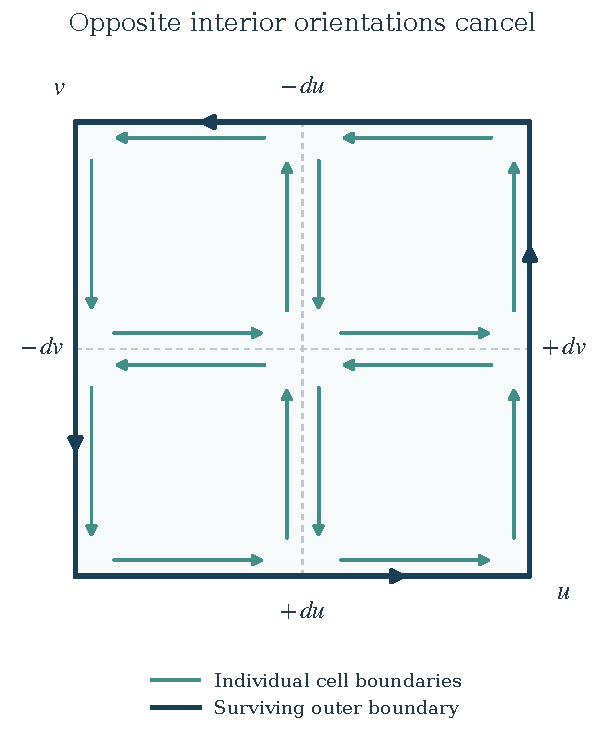
\includegraphics[width=0.52\textwidth]{figures/grid_cancellation.pdf}
\caption{The orientation mechanism in dimension two. Opposite
contributions on a shared grid edge cancel; the outside edges retain
the counterclockwise orientation. The finite telescope proves the
same cancellation in every fixed dimension.}
\label{fig:cancellation}
\end{figure}
\FloatBarrier

\begin{theorem}[Finite Stokes with evaluation errors]\label{thm:finite}
Assume the coordinate remainder certificate
\eqref{eq:derivative-cert}. If $n\ge\tau(t)$, then
\begin{equation}\label{eq:finite-bound}
 \boxed{\quad
 \abs{V_{n,p}-B_{n,p}}
 \le k\,2^{-t}+k(2N+1)2^{-p},\qquad N=2^n .
 \quad}
\end{equation}
\end{theorem}
\begin{proof}
Since $h\le2^{-\tau(t)}$ and each forward edge remains in $Q^k$,
\eqref{eq:derivative-cert} applies to every pair $(a,i)$. Write its residual
as
\[
 R_{a,i}=F_i(x_a+he_i,p)-F_i(x_a,p)-hG_i(x_a,p).
\]
It satisfies
$|R_{a,i}|\le h2^{-t}+(2+h)2^{-p}$.
By \cref{lem:telescoping},
\[
 B_{n,p}-V_{n,p}=h^{k-1}\sum_{a,i}R_{a,i}.
\]
There are precisely $kN^k$ summands. The finite triangle inequality therefore
gives
\begin{align*}
 \abs{B_{n,p}-V_{n,p}}
 &\le h^{k-1}kN^k
             \left(h2^{-t}+(2+h)2^{-p}\right)\\
 &=k2^{-t}+k(2N+1)2^{-p},
\end{align*}
because $N^kh^k=1$ and $N^kh^{k-1}=N$. This uses only finite rational
identities and inequalities.
\end{proof}

\begin{remark}[Why the precision must depend on the mesh]
Exact cancellation of identical samples does not remove the evaluation
term from the \emph{local remainder estimate}. Each comparison with a
derivative involves two coefficient evaluation errors. Summing their
absolute bounds produces $2kN2^{-p}$. Keeping $p$ fixed while increasing $N$
would make this bound worse. The schedule in the next section explicitly
increases $p$ with $n$. The analogous one-dimensional issue is already
identified in the inspected calculus packet \cite{repo-calculus}.
\end{remark}

\subsection{An optional sharper exact-evaluation version}

If the coefficient and derivative values are rational and are evaluated
exactly, and
\[
 \abs{f_i(x+he_i)-f_i(x)-hg_i(x)}\le C_i h^2,
\]
the same proof yields
\[
 \abs{V_N-B_N}\le h\sum_{i=1}^kC_i.
\]
This is useful for polynomial examples. It is not substituted for
\eqref{eq:finite-bound} in the general theorem, where values are available
only through approximation programs.

\FloatBarrier
\section{Constructing the integrals and proving equality}\label{sec:names-proof}

\subsection{A finite refinement lemma}

Let $H(x,p)$ satisfy (C) and (U) on $Q^d$, with modulus $\mu_H$.
Define its left-grid sum
\[
 R_H(n,p)=2^{-nd}\sum_{a\in\Grid{2^n}{d}}H(2^{-n}a,p).
\]
The definition includes $d=0$: the sum has one term and weight one.

\begin{lemma}[Dyadic refinement]\label{lem:refinement}
If $m\ge n\ge\mu_H(t)$, then
\begin{equation}\label{eq:refinement}
 \abs{R_H(n,p)-R_H(m,q)}
 \le2^{-t}+2^{-p}+2^{-q}.
\end{equation}
\end{lemma}
\begin{proof}
Let $L=2^{m-n}$. Every fine index has the unique coordinatewise decomposition
$b=La+c$, with $a\in\Grid{2^n}{d}$ and $c\in\Grid{L}{d}$.
Its fine sample is $2^{-m}b=2^{-n}a+2^{-m}c$. Its distance from the
coarse sample is at most $2^{-n}$, so (U) bounds the difference of the
two sampled values by the right side of \eqref{eq:refinement}.
For each $a$, there are $L^d$ fine points, and
$L^d2^{-md}=2^{-nd}$. Rewrite the coarse sum using those repeated fine
weights, subtract the fine sum, and apply the finite triangle inequality.
The sum of all weights is one. When $d=0$ the same calculation has one
point and uses the zero distance between that point and itself.
\end{proof}

This proof is a grouping identity for finite sums. It invokes neither a
measure-theoretic Fubini theorem nor convergence of an infinite sequence.

\subsection{An integral is an explicitly specified name}

For one coefficient define
\begin{equation}\label{eq:generic-integral-name}
 I_H(r)=R_H\bigl(\max\{r,\bar\mu_H(r+2)\},\,r+2\bigr).
\end{equation}
For $s\ge r$, \cref{lem:refinement} gives
\[
 \abs{I_H(r)-I_H(s)}
 \le 2^{-(r+2)}+2^{-(r+2)}+2^{-(s+2)}
 \le2^{-r}+2^{-s}.
\]
Thus $I_H$ is a primitive recursive regular name. We define
$\int_{Q^d}H$ to be its equality class in the shorthand of
\eqref{eq:name-equality}. The object theory needs only the name and the
formula, not an actual quotient sort.

Any other primitive recursive grid-and-evaluation schedule with an
explicit convergence rate represents the same integral, after
reindexing to a regular name when necessary, if its mesh
eventually satisfies the prescribed modulus and its evaluation precision
tends to infinity with a prescribed rate. Indeed, compare the two dyadic
grids at a target accuracy using \cref{lem:refinement}, taking the smaller
grid first, and then apply \cref{lem:slack}.

Finite linearity follows in the same way. At a common grid and sufficiently
guarded evaluation precision, addition and scalar multiplication are
identities of rational sums; the accumulated approximation error is
bounded by the sum of the coefficient weights. Refinement then proves
the equality of the associated names. In particular a sum of $M$ terms
requires at most an additional $\ell(M)$ precision bits, and an integer
linear combination uses $\ell(\max\{1,\sum|c_j|\})$.

\subsection{One schedule for both sides of Stokes}

Let $\ell=\ell(k)$. Define
\begin{align}
 t_r &= r+\ell+4,\label{eq:schedule-t}\\
 n_r &= \max\{r,\bar\mu_F(t_r),\bar\mu_G(t_r),\bar\tau(t_r)\},
       \label{eq:schedule-n}\\
 p_r &= n_r+t_r+2,\label{eq:schedule-p}\\
 V_r &= V_{n_r,p_r},\qquad B_r=B_{n_r,p_r}.\label{eq:schedule-values}
\end{align}
All functions in this display are primitive recursive. Both $n_r$ and
$p_r$ are nondecreasing. The factor $2^{n_r}$ may be large; the theorem is
about primitive recursive construction, not a polynomial-time algorithm.

\begin{theorem}[Explicit Cauchy and equality rates]\label{thm:rates}
Under (C), (U), and (D), for $s\ge r$,
\begin{align}
 \abs{V_r-B_r}&\le\frac7{64}\,2^{-r},\label{eq:rate-diagonal}\\
 \abs{V_r-V_s}&\le\frac3{32}\,2^{-r},\label{eq:rate-volume}\\
 \abs{B_r-B_s}&\le\frac3{16}\,2^{-r}.\label{eq:rate-boundary}
\end{align}
The functions $V,B$ are regular names, represent the volume and boundary
integrals in \eqref{eq:stokes-intro}, and satisfy $V\EqName B$.
\end{theorem}
\begin{proof}
Put $N=2^{n_r}$. Since $2N+1\le3N$ and
$2^{-p_r}=2^{-n_r}2^{-t_r}/4$, \cref{thm:finite} gives
\[
 \abs{V_r-B_r}
 \le \frac74\,k2^{-t_r}
 \le\frac7{64}\,2^{-r},
\]
where $k\le2^\ell$ was used in the last step.

For the volume sums, apply \cref{lem:refinement} to each $G_i$ and sum.
Since $p_s\ge p_r\ge t_r+2$,
\[
 \abs{V_r-V_s}
 \le k\left(2^{-t_r}+2^{-p_r}+2^{-p_s}\right)
 \le\frac32\,k2^{-t_r}
 \le\frac3{32}\,2^{-r}.
\]
For the boundary sums there are $2k$ restricted coefficient functions.
Face insertion preserves sup-norm distances, so the same modulus
$\mu_F$ applies to each of them. Their total bound is twice the preceding
bound, proving \eqref{eq:rate-boundary}.

These inequalities imply \eqref{eq:regular} after deciding whether $r\le s$
or $s\le r$. The schedules tend to finer meshes and higher precision
explicitly, so \cref{lem:refinement} and finite linearity identify their
names with the integrals defined in \eqref{eq:generic-integral-name}.

Finally let $a,b\ge r$. If $a\le b$, insert $B_a$:
\[
 \abs{V_a-B_b}
 \le\abs{V_a-B_a}+\abs{B_a-B_b}
 \le\left(\frac7{64}+\frac3{16}\right)2^{-a}
 \le\frac{19}{64}\,2^{-r}.
\]
If $b\le a$, insert $V_b$ and obtain the smaller constant
$3/32+7/64=13/64$. This proves \eqref{eq:headline}.
Taking $r=\min\{a,b\}$ also yields
$|V_a-B_b|\le2^{-a}+2^{-b}$ directly. Hence $V\EqName B$.
\end{proof}

\begin{corollary}[Arithmetic form of cubical Stokes]\label{cor:arith-stokes}
For every fixed tuple of primitive recursive evaluators and moduli,
$\ipra$ proves
\[
 \mathsf H(F,G,\mu_F,\mu_G,\tau)\ \longrightarrow\
 \bigl(\mathsf{Name}(V)\wedge\mathsf{Name}(B)\wedge V\EqName B\bigr),
\]
as well as the explicit rational inequalities
\eqref{eq:rate-diagonal}--\eqref{eq:rate-boundary}.
\end{corollary}

The final universal quantifiers range over precision indices and rational
codes. In \cref{sec:ipra-audit} we give the induction invariants and
denominator-clearing procedure that justify the asserted $\ipra$
derivability. No general transfer theorem from constructive analysis to
$\ipra$ is being invoked.

\subsection{Stability under finite perturbations}

If two volume integrands differ pointwise by at most $\eta$ on a unit
cube, their integrals differ by at most $\eta$, with the corresponding
evaluation tolerances added at the finite level. The proof is a weighted
finite triangle inequality, followed by the same named-integral argument.
For a boundary made of $2k$ unit faces the analogous bound is $2k\eta$.
These estimates permit independently certified coefficient approximations
and are also the mechanism by which equal face parameterizations yield
equal face integrals.

\section{Effective calculus needed for curved cells}\label{sec:calculus}

The cube theorem is complete without this section. To apply it to a curved
surface, however, the pulled-back coefficients must themselves have the
required certificates. We now supply the relevant constructions and
proofs. In particular, the chain rule will not be assumed as an
unexplained analytic oracle.

\subsection{Full first-order jets}

Let $D\subseteq\Q^d$ be a closed rational box. A certified $C^1$ presentation
consists of coefficient and derivative evaluators $H,J_1,\ldots,J_d$,
coherence and uniform continuity certificates, integer bounds $A,D_1$
on the named value and each named derivative, and a primitive recursive
remainder modulus $\rho$. Explicitly, the bounds mean
$|H(x,p)|\le A+\epsilon_p$ and $|J_j(x,p)|\le D_1+\epsilon_p$.
For rational $x,y$ in the box, put $h=\|y-x\|_\infty$. The full
remainder condition is
\begin{align}
 h\le2^{-\rho(t)}\quad\Longrightarrow\quad&
 \left|H(y,p)-H(x,p)
             -\sum_{j=1}^dJ_j(x,p)(y_j-x_j)\right|\notag\\
 &\le h2^{-t}+(2+dh)2^{-p}.
 \label{eq:full-jet}
\end{align}
For a coordinate increment only one derivative appears. To derive (D)
rigorously from \eqref{eq:full-jet}, let $R_p$ be that coordinate residual.
Coherence gives
$|R_p-R_q|\le(2+h)(\epsilon_p+\epsilon_q)$.
Applying \eqref{eq:full-jet} at auxiliary precision $q$ therefore gives
\[
 |R_p|\le h\epsilon_t+(2+h)\epsilon_p+
                         \bigl(4+(d+1)h\bigr)\epsilon_q.
\]
On the unit cube $h\le1$, so the last coefficient is at most $d+5$.
Remove that auxiliary slack by \cref{lem:slack}. The resulting bound is
exactly (D), with $(2+h)\epsilon_p$. For another rational box a
primitive recursive integer upper bound on $h$ serves the same purpose.

We use the lighter notation
\begin{equation}\label{eq:jet-semantic}
 f(y)-f(x)=Df(x)(y-x)+R_f(x,y),\qquad
 |R_f(x,y)|\le h2^{-t}
\end{equation}
for the same family of rational assertions after auxiliary evaluation
errors have been eliminated by \cref{lem:slack}. This notation does not
introduce new real-number quantifiers into $\ipra$.

\subsection{Evaluation at named arguments and domain control}\label{sec:composition-eval}

A coordinatewise regular name $a$ for a point of the closed box
$D=\prod_j[\alpha_j,\beta_j]$ can be evaluated inside that box. Use
\[
 \clip_D(z)_j=\min\{\beta_j,\max\{\alpha_j,z_j\}\}.
\]
Clipping is a primitive recursive rational operation. It does not increase
the distance to any point of $D$. A point name is certified to lie in $D$
by the inequalities
$\alpha_j-\epsilon_p\le a_j(p)\le\beta_j+\epsilon_p$ for every $p$.

If $\mu_H$ is a modulus for $H$, define an extension evaluator by
\begin{equation}\label{eq:extension}
 H^\sharp(a,p)=H\bigl(\clip_D(a(q_p)),\,p+3\bigr),\qquad
 q_p=\max\{p+3,\bar\mu_H(p+3)+2\}.
\end{equation}
For $s\ge p$, the two clipped input samples differ by at most
$2^{-q_p}+2^{-q_s}\le2^{1-q_p}\le2^{-\mu_H(p+3)}$.
Applying (U) gives
\[
 |H^\sharp(a,p)-H^\sharp(a,s)|
 \le2^{-(p+3)}+2^{-(p+3)}+2^{-(s+3)}
 \le\epsilon_p+\epsilon_s.
\]
Equivalent input names produce equivalent output names by the same
argument at an increased precision. On a constant rational input this
extension agrees with the original evaluator.

For continuity assertions at named arguments one may conservatively replace
a rational modulus $\mu(t)$ by $\bar\mu(t+2)+2$. This supplies room for
the errors in both input samples. For the full-jet assertion a similar
fixed guard, for example $\bar\rho(t+2)+2$, ensures that rational
approximants lie within the required remainder radius. Approximate all
arguments, apply the rational certificate, and use \cref{lem:slack} to
remove the auxiliary errors. The sup norm, finite products, and finite sums
are continuous with the explicit error propagation given below, so this
procedure is entirely finite arithmetic at each precision.

In the remaining formulas, $\rho$ and $\mu$ refer to valid moduli for
these guarded named-argument statements. All displayed majorants remain
primitive recursive after this fixed guarding. If an implementation works
only with rational samples of an expression, the same guard can instead be
inserted during expression compilation.

This detail matters: a rational approximation to $\sigma(x)$ can fall just
outside a box that contains the exact image. Evaluating an ambient
coefficient there without a domain certificate would be unjustified.
Clipping avoids that issue. It is used only in the approximation algorithm;
we do not differentiate the clipping operation. The named composition is
the composition with $\sigma$, whose range is certified to be in $D$.

\subsection{A finite evaluator for arithmetic expressions}

Suppose represented quantities $a,b$ have known absolute bounds $A,B$.
For a sum, evaluate both at precision $p+1$. For a product, evaluate both
at
\[
 q=p+\ell(A+B+1).
\]
If $|\widetilde a-a|,|\widetilde b-b|\le2^{-q}$, then
\[
 |\widetilde a\widetilde b-ab|
 \le A2^{-q}+B2^{-q}+2^{-2q}
 \le(A+B+1)2^{-q}\le2^{-p}.
\]
Bounds for new exact values are $A+B$ and $AB$. Subtraction uses sign
reversal and addition. A finite sum uses the sum of its term bounds and
a precision shift $\ell(M)$ for $M$ terms. Each determinant is evaluated
using its finite permutation expansion.

These recursive instructions assign both a bound and an evaluation
precision to every node of a fixed arithmetic expression tree. Composition
uses \eqref{eq:extension}. Hence all expressions used in pullback and
exterior differentiation have primitive recursive evaluators with
specified error budgets. Coherence and preservation of equality follow
from the corresponding finite error inequalities and
\cref{lem:slack}.

\subsection{A local Lipschitz estimate without a mean-value theorem}

If the derivatives of a $d$-variable presentation are bounded by $D_1$,
\eqref{eq:jet-semantic} at $t=0$ gives
\begin{equation}\label{eq:local-lip}
 |f(y)-f(x)|\le(dD_1+1)h
 \qquad(h\le2^{-\rho_f(0)}).
\end{equation}
Thus
\[
 \mu_f(t)=\max\{\rho_f(0),\ t+\ell(dD_1+1)\}
\]
is an explicit value-continuity modulus. This direct estimate is enough
for every closure proof below. No existence of a maximum, mean-value
point, or integral is involved.

\subsection{Sums and products}\label{sec:product}

For $f+g$, add their jets. Use
$\rho_{f+g}(r)=\max\{\rho_f(r+1),\rho_g(r+1)\}$.
Negation preserves the modulus. The corresponding value and derivative
continuity moduli follow by the same precision shift.

For products suppose
\[
 |f|\le A_f,\quad |g|\le A_g,\quad
 |\partial_jf|\le D_f,\quad|\partial_jg|\le D_g.
\]
Put $L_f=dD_f+1$, $L_g=dD_g+1$, and take all remainder moduli to be
nondecreasing. Writing $\Delta f=f(y)-f(x)$ and similarly for $g$, direct
expansion gives
\begin{align}
 &(fg)(y)-(fg)(x)
       -\sum_j(g\,\partial_jf+f\,\partial_jg)(x)(y_j-x_j)\notag\\
 &\hspace{2em}=g(x)R_f+f(x)R_g+\Delta f\,\Delta g.
 \label{eq:product-remainder}
\end{align}
When both jets are valid at accuracy $t$ and their local Lipschitz estimates
apply, the absolute value is at most
\[
 h(A_f+A_g)2^{-t}+h^2L_fL_g.
\]
For a desired remainder accuracy $r$, set
\begin{align}
 t&=r+\ell\bigl(2(A_f+A_g+1)\bigr),\notag\\
 \rho_{fg}(r)
 &=\max\{\rho_f(t),\rho_g(t),\,r+\ell(2L_fL_g)\}.
 \label{eq:product-modulus}
\end{align}
The first term of the remainder is at most $h2^{-r}/2$, and the second
is at most $h2^{-r}/2$. Since $t\ge0$ and the moduli are monotone,
the local Lipschitz radii at accuracy zero are automatically respected.
This proves the product rule and its full uniform remainder certificate.

The product derivative is bounded by $A_gD_f+A_fD_g$. If a common
modulus for $f$ and its first derivatives is $\mu_f$, and similarly for
$g$, put
\[
 s=r+\ell(A_f+A_g+D_f+D_g+1).
\]
The modulus $\max\{\mu_f(s),\mu_g(s)\}$ controls the variation of each
product derivative: expand its two product differences, obtaining four
terms with total coefficient bound
$A_f+A_g+D_f+D_g$. This supplies the required derivative-continuity
certificate as well as the remainder certificate.

\subsection{Composition and its chain rule}\label{sec:chain-rule}

Let $f$ have $m$ inputs with $|\partial_af|\le D$, and let
$\sigma:Q^k\to D$ have componentwise $C^1$ jets with
$|\partial_i\sigma_a|\le M$. The image containment in the rational box is
part of the certificate. Let $\rho_\sigma$ majorize the component
remainder moduli and put $L=kM+1$.

For $\delta=\|y-x\|_\infty\le2^{-\rho_\sigma(0)}$,
\eqref{eq:local-lip} gives $\|\sigma(y)-\sigma(x)\|_\infty\le L\delta$.
Expand both jets:
\[
 \Delta\sigma=D\sigma(x)(y-x)+R_\sigma,\qquad
 f(\sigma(y))-f(\sigma(x))
   =Df(\sigma(x))\Delta\sigma+R_f.
\]
Subtracting the proposed chain-rule term leaves
$Df(\sigma(x))R_\sigma+R_f$. If the component remainders of $\sigma$
are at accuracy $u$, and the remainder of $f$ is at accuracy $t$, this
is bounded by
\begin{equation}\label{eq:composition-remainder}
 mD\,\delta\,2^{-u}+L\delta\,2^{-t}.
\end{equation}
For target accuracy $r$, choose
\begin{align}
 t&=r+\ell(2L),&
 u&=r+\ell\bigl(2(mD+1)\bigr),\notag\\
 \rho_{f\circ\sigma}(r)
 &=\max\{\rho_\sigma(0),\rho_\sigma(u),
                     \rho_f(t)+\ell(L)\}.
 \label{eq:composition-modulus}
\end{align}
The last condition ensures $L\delta\le2^{-\rho_f(t)}$; the other
conditions validate the two jets. Equation
\eqref{eq:composition-remainder} is at most $\delta2^{-r}$. Therefore
\begin{equation}\label{eq:chain-rule}
 \partial_i(f\circ\sigma)
 =\sum_{a=1}^m(\partial_af)\circ\sigma\,\partial_i\sigma_a
\end{equation}
with the explicit remainder modulus just given.

For completeness, derivative continuity can also be computed directly.
The derivative bound is $mDM$. In the difference of the two sums in
\eqref{eq:chain-rule}, there are $m$ product differences, with total
coefficient bound $m(M+D)$. Put
$s=r+\ell(m(M+D)+1)$. A valid modulus is the maximum of
$\rho_\sigma(0)$, the modulus for $D\sigma$ at $s$, and
the modulus for $Df$ at $s$ plus $\ell(L)$. This ensures that the
variation of every factor has the required accuracy. A value-continuity
modulus follows from \eqref{eq:local-lip} for the newly constructed jet.

The proof of \eqref{eq:chain-rule} is an algebraic expansion with finite
bounds. If named arguments occur, approximate them at an auxiliary
precision, apply these rational expansions and the expression evaluator,
and remove the final rational slack. It therefore has the same
first-order arithmetic interpretation as the cube proof.

\subsection{Second jets and symmetry}

A certified $C^2$ parameterization contains a $C^1$ jet for every
component $\sigma_a$, a $C^1$ jet for every first derivative
$\partial_i\sigma_a$, and the named equalities
\[
 H^a_{ij}=H^a_{ji},\qquad
 H^a_{ij}=\partial_i(\partial_j\sigma_a).
\]
Bounds and uniform moduli for all these finitely many fields are supplied.
Thus symmetry of the second jet is an explicit part of this presentation.
We do not silently invoke a classical theorem about interchanging
partials. Polynomial and expression-generated examples have symmetry
proofs by their finite algebraic differentiation rules. To admit a weaker
input interface containing only nonsymmetric proposed partial derivatives,
one would first need to prove the appropriate quantitative rectangular
increment theorem; that extra interface is not used here.

The following section needs exactly this much regularity: each first
derivative of $\sigma$ must have a first jet, and its antisymmetric second
part must vanish. An immersion lower bound is unnecessary for the
parameterized-chain identity.

\subsection{Polynomial certificates without integration}\label{sec:polynomial-jets}

There are many nonvacuous inputs for these interfaces. Let
$P(x)=\sum_\alpha c_\alpha x^\alpha$ be a rational polynomial on a box
$|x_j|\le R$, with integer $R\ge1$, total degree at most $D$, and integer
$A\ge\sum_\alpha|c_\alpha|$. Exact rational evaluation is primitive
recursive. Differentiation of its finite coefficient list is primitive
recursive too.

For $\|\Delta\|_\infty=h\le1$, expand each monomial by the multivariate
binomial identity. The constant and linear terms are $P(x)$ and
$DP(x)\Delta$. Every remaining term has at least two factors from
$\Delta$, hence contains $h^2$ as a bound. Summing their absolute values gives
\begin{equation}\label{eq:polynomial-jet}
 \abs{P(x+\Delta)-P(x)-DP(x)\Delta}
 \le A(R+1)^D h^2.
\end{equation}
Indeed the full binomial coefficient sum for a monomial of degree $d$
is bounded by $(R+1)^d\le(R+1)^D$.
Consequently
\[
 \rho_P(r)=r+\ell\bigl(\max\{1,A(R+1)^D\}\bigr)
\]
is a remainder modulus.

Bounds $AR^D$, $ADR^D$, and $AD^2R^D$ suffice for values, first
derivatives, and second derivatives. Continuity bounds can be derived
from the elementary product-difference identity for monomials: their
variation is at most their degree times $R$ to an appropriate power,
times $\|\Delta\|_\infty$. A common safe Lipschitz bound for the value
and its first derivatives is $A(D+1)^2R^D$. The second derivatives
are handled by differentiating the finite polynomial again. All these
claims are finite coefficient identities and inequalities; no FTC or
Stokes theorem is needed to validate them.

\section{Differential forms, pullbacks, and finite chains}\label{sec:geometry}

\subsection{Finite exterior algebra}

For a fixed ambient dimension $m$, a $q$-form is a finite coefficient array
\[
 \omega=\sum_{\substack{I=(i_1<\cdots<i_q)\\1\le i_j\le m}}
                   a_I\,\dd y_{i_1}\wedge\cdots\wedge\dd y_{i_q}.
\]
For $q=0$ the index list is empty and a form is a scalar coefficient.
Multiplication of basis words is defined as follows: concatenate their
index lists; if an index repeats, the product is zero; otherwise sort the
list and multiply by the sign $(-1)^{\text{number of inversions}}$.
This defines the wedge product by finite distributivity. Sorting,
duplicate detection, and inversion counting are all bounded operations.

For $C^1$ coefficients, the exterior derivative is defined by
\[
 \dd\omega=\sum_I\sum_{a=1}^m
          \partial_a a_I\,\dd y_a\wedge\dd y_{i_1}\wedge\cdots\wedge\dd y_{i_q}.
\]
Equivalently, its coefficient at $K=(k_1<\cdots<k_{q+1})$ is
\[
 (\dd\omega)_K
   =\sum_{\nu=1}^{q+1}(-1)^{\nu-1}
        \partial_{k_\nu}a_{K\setminus k_\nu}.
\]
These formulas specify all signs without a topological convention left
implicit.

Finite expansion and the scalar product rule prove the graded Leibniz
identity
\[
 \dd(\alpha\wedge\beta)
 =\dd\alpha\wedge\beta+(-1)^{\deg\alpha}\alpha\wedge\dd\beta.
\]
Indeed, differentiating a coefficient product produces its two scalar
terms. In the second term the new one-form must move past
$\deg\alpha$ basis one-forms, giving the displayed sign. Repeated-index
terms vanish in both expansions. This is a finite matching of coefficient
terms.

\subsection{The pullback construction}

Let $\sigma:Q^k\to D\subseteq\R^m$ be a certified parameterization.
Define
\[
 \dd\sigma_a=\sum_{j=1}^k\partial_j\sigma_a\,\dd x_j,\qquad
 \sigma^*\omega=\sum_I(a_I\circ\sigma)
                  \dd\sigma_{i_1}\wedge\cdots\wedge\dd\sigma_{i_q}.
\]
For an increasing parameter index list $J$ of length $q$, the coefficient
is
\begin{equation}\label{eq:pullback-minors}
 (\sigma^*\omega)_J
 =\sum_{|I|=q}(a_I\circ\sigma)
        \det\bigl(\partial_{j_b}\sigma_{i_a}\bigr)_{1\le a,b\le q}.
\end{equation}
The determinant here means its permutation expansion. Its construction
requires no inverse matrix or rank decision.

If $\omega$ has certified $C^1$ coefficients and $\sigma$ has a certified
$C^2$ jet, every factor in \eqref{eq:pullback-minors} has a $C^1$
presentation: use the composition lemma for $a_I\circ\sigma$, and the
supplied second jets for $\partial_j\sigma_a$. Apply the sum and product
lemmas finitely many times. This constructs the complete $C^1$ certificate
for the pullback.

For explicit size bounds, suppose a common integer $M\ge1$ bounds all
ambient coefficient values and first derivatives, and all first and
second derivatives of $\sigma$. Then
\[
 \binom mq q!M^{q+1}
\]
bounds every pullback coefficient. A safe bound on any of its first
derivatives is
\[
 \binom mq q!(m+q+1)M^{q+2}.
\]
To see the latter, a derivative falling on $a_I\circ\sigma$ gives at most
$m$ terms; a derivative falling on a determinant gives at most $q$ terms
per permutation. Each term is a product of the bounded factors. This
bound also covers $q=0$. The effective modulus construction is the finite
expression-tree recursion of \cref{sec:product,sec:chain-rule}.

\begin{lemma}[Naturality of the exterior derivative]\label{lem:naturality}
For these certified presentations,
\[
 \dd(\sigma^*\omega)=\sigma^*(\dd\omega)
\]
as coefficientwise equality of named forms.
\end{lemma}
\begin{proof}
First,
\[
 \dd(\dd\sigma_a)
 =\sum_{i<j}
   \bigl(\partial_i\partial_j\sigma_a
          -\partial_j\partial_i\sigma_a\bigr)\dd x_i\wedge\dd x_j=0
\]
by the symmetry certificates for the second jet. For one summand of
$\sigma^*\omega$, apply the graded product rule:
\begin{align*}
 &\dd\bigl((a_I\circ\sigma)
                  \dd\sigma_{i_1}\wedge\cdots\wedge\dd\sigma_{i_q}\bigr)\\
 &\quad=\dd(a_I\circ\sigma)
                  \wedge\dd\sigma_{i_1}\wedge\cdots\wedge\dd\sigma_{i_q}.
\end{align*}
All the other terms contain a factor $\dd(\dd\sigma_{i_j})$ and vanish.
By the chain rule already proved,
$\dd(a_I\circ\sigma)=\sum_a(\partial_a a_I\circ\sigma)\dd\sigma_a$.
Substitution gives exactly the pullback of
$\sum_a\partial_a a_I\,\dd y_a\wedge\dd y_I$. Sum over $I$.
Every equality is a finite coefficient expansion, using the explicit
jet closure lemmas, and no integration theorem has entered the proof.
\end{proof}

\subsection{Integrating a parameterized cell}

For a $k$-form $\eta$ with certified uniformly continuous coefficients,
define
\[
 \int_\sigma\eta:=\int_{Q^k}\sigma^*\eta.
\]
The right side is the named integral of its single top-degree coefficient.
For $\eta=\dd\omega$, the supplied first-derivative continuity of
$\omega$ provides this condition; a second derivative of the ambient
form is not required.
The boundary of $\sigma$ is the formal chain
\begin{equation}\label{eq:sigma-boundary}
 \partial\sigma
 =\sum_{i=1}^k(-1)^{i-1}
         \bigl(\sigma\circ\delta_i^1-\sigma\circ\delta_i^0\bigr).
\end{equation}
For a zero-dimensional cell, integration of a zero-form is its value
at the point, and its boundary is zero.

Restriction of a jet to a face merely deletes the frozen coordinate
directions; its moduli and bounds can be retained. Direct substitution
in the finite minor formula proves
\[
 (\sigma\circ\delta_i^\varepsilon)^*\omega
       =(\delta_i^\varepsilon)^*(\sigma^*\omega).
\]
Thus the boundary integral defined from \eqref{eq:sigma-boundary} is the
boundary integral of the pulled-back form, with exactly the signs used
in the cube theorem.

\begin{theorem}[Stokes for a certified curved cube]\label{thm:curved}
Let $\sigma$ be a certified $C^2$ $k$-cube in a rational ambient box, and
let $\omega$ be a certified $C^1$ $(k-1)$-form there. Then
\[
 \int_\sigma\dd\omega\ \EqName\ \int_{\partial\sigma}\omega .
\]
The pullback construction and the schedule
\eqref{eq:schedule-t}--\eqref{eq:schedule-values} give primitive recursive
names and explicit equality witnesses.
\end{theorem}
\begin{proof}
The effective calculus constructs the $C^1$ coefficient presentation of
$\alpha=\sigma^*\omega$. Write it in flux form \eqref{eq:flux-form}.
Its diagonal derivative data satisfy (D), and all coefficients and
diagonal derivatives satisfy (C) and (U). Apply \cref{thm:rates}.
By \cref{lem:naturality}, the volume side is
$\int_{Q^k}\sigma^*(\dd\omega)=\int_\sigma\dd\omega$.
The face-restriction identity identifies the boundary side with
$\int_{\partial\sigma}\omega$.
\end{proof}

\subsection{Finite chains and the error budget}

Define the integral over $C=\sum_{\lambda<L}c_\lambda\sigma_\lambda$
by the same finite integer linear combination of integrals, and define
$\partial C=\sum c_\lambda\partial\sigma_\lambda$. Put
$W=\sum_{\lambda<L}|c_\lambda|$. If $W=0$, both sides are zero.
Otherwise let $s=\ell(W)$ and define
\[
 V_C(r)=\sum_{\lambda<L}c_\lambda V_\lambda(r+s),\qquad
 B_C(r)=\sum_{\lambda<L}c_\lambda B_\lambda(r+s).
\]
Here the individual names are those in \cref{thm:curved}. The finite
triangle inequality multiplies every bound by at most $W$, and
$W2^{-s}\le1$. Hence the Cauchy and equality rates of
\cref{thm:rates} remain valid for $V_C,B_C$. This proves
\cref{thm:informal}. One can use separate meshes for separate cells,
or take the finite maximum of their moduli and use a common mesh.

\subsection{Why the boundary has no boundary}

Faces can be represented by the original cell identifier and a sorted
list of frozen original coordinates with their endpoint values.
This representation makes two successive face restrictions normalize
to the same data when they freeze the same two coordinates.

Fix original coordinates $i<j$ and endpoint values
$\varepsilon,\eta$. Freezing $i$ first makes the later index for $j$
equal to $j-1$. Its sign in the double boundary is
\[
 (-1)^{i-1+j-2}(2\varepsilon-1)(2\eta-1).
\]
Freezing $j$ first leaves the later index for $i$ equal to $i$.
The sign is
\[
 (-1)^{j-1+i-1}(2\eta-1)(2\varepsilon-1),
\]
which is its negative. Each codimension-two face occurs exactly in
these two ways. Their coefficients cancel, proving
\[
 \partial^2C=0
\]
by a finite sign-reversing pairing. No decision procedure for extensional
equality of arbitrary parameterization programs is required.

\subsection{Matching faces and orientation changes}

For different cells, the fact that two geometric faces coincide is not
decided by comparing arbitrary programs. An interface matching record
may instead supply an explicit equality of their parameterizations and
tangential first jets, with named equality witnesses. The continuity
and finite-expression bounds then prove equality of their pulled-back
coefficients. If their signed multiplicities are opposite, their
integrals cancel.

A useful supported reparameterization is a permutation and reflection
of cube coordinates. Let $T:Q^d\to Q^d$ be such a signed coordinate
permutation, with constant determinant $s\in\{-1,1\}$. The midpoint
grid $\{(a+\tfrac12)/N\}$ is permuted exactly by $T$. For a top form
$b(x)\,\dd x_1\wedge\cdots\wedge\dd x_d$, the rational midpoint sums
for its pullback, using the direct valid evaluator
$H_T(x,p)=sH(Tx,p)$, are therefore exactly $s$ times the original sums.
The general guarded composition evaluator is equivalent to this one,
although it need not return the same rational sample at the same
precision. Uniform coefficient equality identifies their integral names.
The midpoint and left-grid sums are within the same (U) bound,
because corresponding tags are at distance at most $1/N$.
Their names agree by refinement. Consequently
\[
 \int_{Q^d}T^*\eta=s\int_{Q^d}\eta.
\]
This proves the orientation rule needed for matching faces after a
coordinate symmetry. A matching record must include this sign.

Dyadic subdivision also preserves an integral: use direct rational affine
evaluation and the exact determinant weight on each subcube. The
resulting points and weights are exactly those in the refined whole-cube
sum. Finite grouping proves the identity, and the guarded evaluator
represents the same named integral. Thus many
presentation changes can be certified without a general
change-of-variables theorem. Invariance under an arbitrary smooth
diffeomorphism is a separate theorem and is not silently assumed here.

\section{Classical vector-calculus forms}\label{sec:vector}

\subsection{Kelvin--Stokes on a surface patch}

Let $\sigma(u,v)=(\sigma_1,\sigma_2,\sigma_3)$ be a certified $C^2$ patch,
and let $\mathbf F=(F_1,F_2,F_3)$ have a certified $C^1$ jet.
For $\omega=F_1\dd x+F_2\dd y+F_3\dd z$ set
\[
 P=\mathbf F(\sigma)\cdot\sigma_u,\qquad
 Q=\mathbf F(\sigma)\cdot\sigma_v.
\]
Then $\sigma^*\omega=P\,\dd u+Q\,\dd v$. The flux coefficients of
the cube theorem are $f_1=Q$ and $f_2=-P$.

The product and chain rules give
\begin{align*}
 \partial_uQ-\partial_vP
 &=\sum_{a,b}(\partial_aF_b)(\sigma)
       \bigl((\partial_u\sigma_a)(\partial_v\sigma_b)
             -(\partial_v\sigma_a)(\partial_u\sigma_b)\bigr).
\end{align*}
Terms containing $F_b(\sigma)\partial_u\partial_v\sigma_b$ cancel
by the second-jet symmetry. Expanding the three-component cross
product shows that the remaining finite polynomial is
\[
 (\curl\mathbf F)(\sigma)\cdot(\sigma_u\times\sigma_v).
\]
Therefore \cref{thm:curved} becomes
\begin{align}
 &\int_0^1P(u,0)\,\dd u+\int_0^1Q(1,v)\,\dd v
       -\int_0^1P(u,1)\,\dd u-\int_0^1Q(0,v)\,\dd v\notag\\
 &\hspace{2em}=
 \int_{Q^2}(\curl\mathbf F)(\sigma(u,v))
                       \cdot(\sigma_u\times\sigma_v)\,\dd u\,\dd v .
 \label{eq:kelvin-explicit}
\end{align}
All equalities in this section are equalities of the constructed names.
The boundary runs counterclockwise in the parameter square.

For an embedded oriented surface given by compatible patches, the right
side is the usual oriented surface integral, and the matched interior
edges cancel. The vector area element is used directly:
$\mathbf n\,\dd S=(\sigma_u\times\sigma_v)\dd u\,\dd v$.
There is no need to divide by $|\sigma_u\times\sigma_v|$ or compute a unit
normal. An immersion certificate is needed only for the additional
geometric interpretation as a regular embedded patch, not for the
parameterized identity itself.

\subsection{Green, divergence, and exact-form consequences}

For a planar patch, $\omega=P\,\dd x+Q\,\dd y$ gives
\[
 \int_{\partial C}P\,\dd x+Q\,\dd y
   =\int_C(\partial_xQ-\partial_yP)\,\dd x\wedge\dd y.
\]
For a three-dimensional chain use
\[
 \omega=F_1\,\dd y\wedge\dd z
       +F_2\,\dd z\wedge\dd x+F_3\,\dd x\wedge\dd y.
\]
Its exterior derivative is
$(\partial_xF_1+\partial_yF_2+\partial_zF_3)\dd x\wedge\dd y\wedge\dd z$,
giving the divergence theorem for the supplied presentation.
For $k=1$, the theorem is the fundamental theorem of calculus for
certified parameterized paths; only $C^1$ path data are needed in that
case.

If $\partial C=0$, then $\int_C\dd\eta=0$ whenever the indicated
certificates are available. If $C_1-C_2=\partial D$ is a \emph{supplied}
finite filling and $\dd\omega=0$ with a certificate, then
$\int_{C_1}\omega=\int_{C_2}\omega$.
These are constructive consequences of finite chain algebra and the
proved Stokes identity. They do not assert the existence of a filling
or solve a topological recognition problem.

\section{A complete curved polynomial example}\label{sec:example}

Consider the upward-oriented patch
\[
 \sigma(u,v)=(u,v,uv),\qquad 0\le u,v\le1,
\]
and the vector field
\[
 \mathbf F(x,y,z)=(0,xz,x^2y).
\]
These are rational polynomials on the relevant unit boxes. Exact evaluation,
all derivative programs, and the certificates of
\cref{sec:polynomial-jets} are available by finite arithmetic.
The normal area vector is
\[
 \sigma_u=(1,0,v),\qquad \sigma_v=(0,1,u),\qquad
 \sigma_u\times\sigma_v=(-v,-u,1).
\]
Its third coordinate is one, so there is no degeneracy or orientation
ambiguity in this particular surface presentation.

\subsection{Pullback and curl calculation}

The pulled-back one-form is
\[
 \sigma^*(\mathbf F\cdot\dd\mathbf r)=P\,\dd u+Q\,\dd v,
 \qquad
 P=u^2v^2,\qquad Q=u^2v(1+u).
\]
Indeed $\mathbf F(\sigma)=(0,u^2v,u^2v)$, and taking its dot products
with the two tangent vectors gives these expressions.
Differentiating the finite polynomials gives
\[
 \partial_uQ-\partial_vP=(2u+3u^2)v-2u^2v=uv(u+2).
\]
Independently,
\[
 \curl\mathbf F=(x^2-x,-2xy,z),
\]
and
\[
 (\curl\mathbf F)(\sigma)\cdot(-v,-u,1)
 =-(u^2-u)v+2u^2v+uv=uv(u+2).
\]
This checks both curvature and a nonconstant curl integrand; it is not
an example in which the surface dependence disappears trivially.

\subsection{Boundary values and exact integral}

The four counterclockwise edges give
\[
 \begin{array}{c|c|c}
 \text{edge}&\text{oriented integrand}&\text{integral}\\ \hline
 v=0,\ u:0\to1&0&0\\
 u=1,\ v:0\to1&2v&1\\
 v=1,\ u:1\to0&-u^2\text{ on }[0,1]&-1/3\\
 u=0,\ v:1\to0&0&0
 \end{array}
\]
Thus the boundary integral is $2/3$. The volume side is also $2/3$.
This statement can be checked without assuming ordinary integration
formulas: the following finite-sum identities explicitly construct the
two names and their common rational value.

\subsection{Every Riemann sum in closed form}

Use exact evaluation and $N$ equal intervals in each parameter direction.
The finite identities
\[
 \sum_{a<N}a=\frac{N(N-1)}2,\qquad
 \sum_{a<N}a^2=\frac{N(N-1)(2N-1)}6
\]
are proved by quantifier-free induction after clearing denominators.
Substitution in the definitions of $V$ and $B$ yields
\begin{align}
 V_N&=\frac{(N-1)^2(8N-1)}{12N^3},\label{eq:example-V}\\
 B_N&=\frac{(N-1)(4N+1)}{6N^2},\label{eq:example-B}\\
 B_N-V_N&=\frac{(N-1)(11N-1)}{12N^3}.\label{eq:example-defect}
\end{align}
In particular, the two sums are generally different at a finite mesh.
Stokes is equality of their represented integrals, not an assertion that
the derivative Riemann sum equals the boundary Riemann sum at every mesh.
The difference sum $T_N$, in contrast, equals $B_N$ exactly.

The exact errors relative to the common value are
\[
 \frac23-V_N=\frac{17N^2-10N+1}{12N^3},\qquad
 \frac23-B_N=\frac{3N+1}{6N^2}.
\]
For $N\ge1$ these are nonnegative and at most $17/(12N)$ and $2/(3N)$,
respectively. Taking $N\ge2^{r+1}$ makes each error smaller than $2^{-r}$.
This directly verifies the named integral value $2/3$.

\begin{table}[ht]
\centering
\caption{Exactly computed left-grid sums for the curved example.
The decimal columns are only for readability; the validation uses fractions.}
\begin{tabular}{r r r r}
\toprule
$N$&$V_N$&$B_N=T_N$&$B_N-V_N$\\
\midrule
2&0.156250000&0.375000000&0.218750000\\
4&0.363281250&0.531250000&0.167968750\\
8&0.502441406&0.601562500&0.099121094\\
16&0.581359863&0.634765625&0.053405762\\
32&0.623207092&0.650878906&0.027671814\\
\bottomrule
\end{tabular}
\end{table}

\begin{figure}[htbp]
\centering
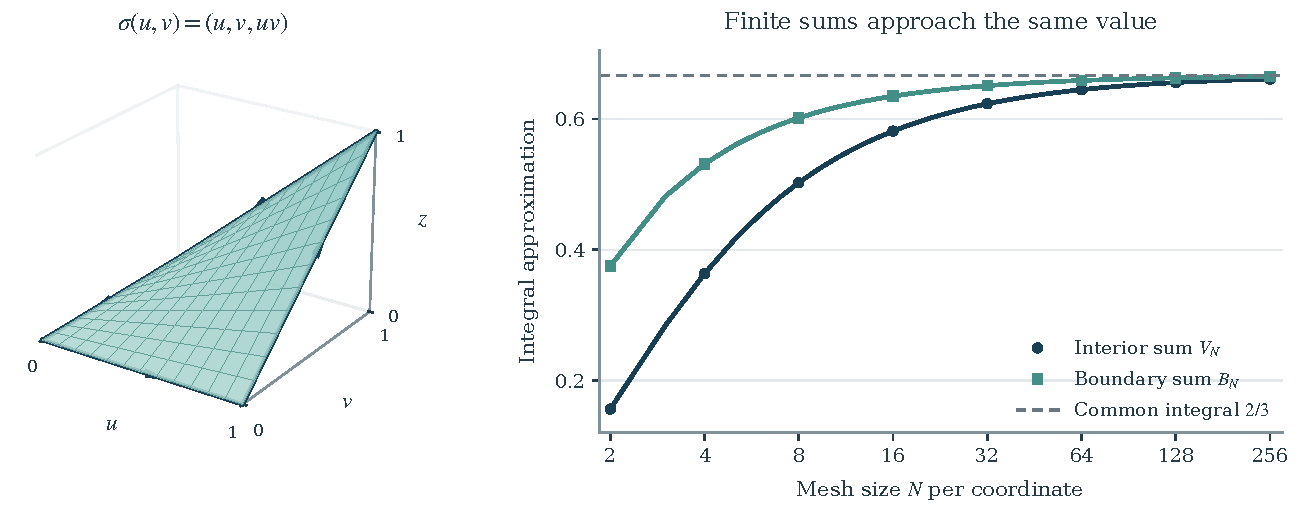
\includegraphics[width=\textwidth]{figures/example_convergence.pdf}
\caption{The curved polynomial patch and its two independently defined
Riemann sums. The common target $2/3$ and the plotted values follow from
the exact rational formulas \eqref{eq:example-V} and \eqref{eq:example-B}.}
\label{fig:example}
\end{figure}

\subsection{Explicit certificates for this example}

The cube flux coefficients and their relevant derivatives are
\[
 f_1=u^2v+u^3v,\quad f_2=-u^2v^2,\quad
 g_1=(2u+3u^2)v,\quad g_2=-2u^2v.
\]
On $Q^2$, their sup-norm Lipschitz bounds are respectively $7,4,13,6$.
For example, on $[0,1]$ the factorization of $a^j-b^j$ gives
$|a^j-b^j|\le j|a-b|$; applying it to each factor in a monomial proves
these constants directly. A common continuity modulus is therefore
\[
 \mu_F(t)=\mu_G(t)=t+4.
\]
Their exact coordinate remainders are
\[
 R_1=vh^2(1+3u+h),\qquad R_2=-u^2h^2.
\]
For an admissible forward $u$-increment, $u+h\le1$, so
$1+3u+h\le4$. Hence $|R_1|\le4h^2$ and $|R_2|\le h^2$.
A common modulus is $\tau(t)=t+2$.

For $k=2$, $\ell(k)=1$, and the general schedule becomes
\[
 t_r=r+5,\qquad n_r=r+9,\qquad N_r=2^{r+9},\qquad p_r=2r+16.
\]
The general finite error budget simplifies exactly to
\[
 \frac{2\,2^{-t_r}+2(2N_r+1)2^{-p_r}}{2^{-r}}
       =\frac3{32}+2^{-r-15}<\frac18.
\]
The exact polynomial values make the evaluation part unnecessary in this
example, so this general bound is deliberately conservative. Its purpose
is to demonstrate the uniform recipe that also works with rounded
coefficient data.

\FloatBarrier
\section{Executable checks and their limits}\label{sec:checks}

The archive contains a Python reference implementation using the standard
library's \path{fractions.Fraction}. It evaluates the finite expressions
$V,B,T$, polynomial coefficients, and cubical boundaries. The independent
validation run recorded the following successful checks:

\begin{center}
\begin{tabular}{p{0.68\textwidth}r}
\toprule
Check & Cases\\
\midrule
Exact telescoping on arbitrary rational sampled tables in dimensions
$1$ through $4$ &36\\
Cancellation of every codimension-two coefficient in $\partial^2$
for dimensions $2$ through $6$ &5\\
Direct enumeration of the curved example at $N=1,2,4,8,16,32$,
compared with the closed formulas &6\\
Rounded dyadic evaluations satisfying the local remainder contract
and the global error bound &48\\
Large precision schedules checked by the independently verified
closed formulas &19\\
\bottomrule
\end{tabular}
\end{center}

The polynomial recurrence identities, the pullback/curl identity, and
the two displayed Taylor remainders were checked by equality of complete
finite coefficient dictionaries. They were not inferred from agreement
at sampled points. The large schedule cases use the closed formulas;
their enormous grids were not enumerated.

These checks catch orientation, scaling, endpoint, and precision-accounting
errors. They are not proofs of a universally quantified theorem, and they
do not replace the human proof or an internal iPRA derivation. Python
callables are an execution interface; the proof-theoretic claim applies
to their fixed primitive recursive mathematical instances.

The JSON receipt includes the source hashes and the exact fractions.
The CSV tables contain the direct-grid and schedule results.
The plotting script is a separate optional dependency on Matplotlib;
the validation itself has no external Python dependencies.

\section{Why the proof fits inside iPRA}\label{sec:ipra-audit}

Primitive recursiveness of an algorithm alone would not prove its claimed
correctness in $\ipra$. The relevant point is that the correctness
arguments above use particular finite induction invariants available
in that theory. We record them and the translation into natural-number
arithmetic.

\subsection{The exact first-order assertion}

Fix all evaluator and modulus programs, allowing an optional tuple of
number parameters $a$. Each rational expression $V(a,r)$ or $B(a,r)$
has a primitive recursive code. Write $\mathsf H(a)$ for the universal
arithmetic certificates in \cref{sec:certificates}.
The main precision assertion is the first-order formula
\begin{equation}\label{eq:object-statement}
 \mathsf H(a)\ \longrightarrow\
 \forall r,u,v\,
 \left(r\le u\wedge r\le v\ \longrightarrow\
       64\,2^r\,|V(a,u)-B(a,v)|\le19\right).
\end{equation}
The displayed rational inequality is expanded into a natural-number
comparison after multiplication by positive denominators. The corresponding
formulas for regularity and equality are expanded in the same way.

There is no internal quantifier over real-valued functions in
\eqref{eq:object-statement}. There is no assertion that a single natural
number codes and evaluates every possible primitive recursive program.
For each fixed syntactic instance, the newly constructed names are
themselves fixed primitive recursive definitions. This is the usual
schematic use of the full primitive recursive language.

\subsection{Clearing denominators and handling negative values}

For one requested finite grid, list the rational quantities needed in
the proof: coefficient samples, width-weighted derivative samples,
grid weights, and error terms. Let $D$ be the product of their positive
denominators. There are primitive recursive bounds on the length of
this list, and its construction is a bounded loop over the grid.
Thus $D$ is a positive primitive recursive integer.

After multiplication by $D$, a coordinate line has integer potential
samples $A(j)$, integer derivative increments $b(j)$, and a nonnegative
integer error $E$. Its local contract has the two forms
\[
 A(j+1)-A(j)-b(j)\le E,\qquad
 b(j)-A(j+1)+A(j)\le E.
\]
To use a natural-valued finite-FTC module, set
\[
 L=\max_{j\le N}\max\{0,-A(j)\},\quad
 G(j)=A(j)+L,\quad b(j)=b^+(j)-b^-(j)
\]
on the guarded range $j\le N$. One may totalize $G$ outside that range
using $\max\{0,A(j)+L\}$.
Then $G,b^+,b^-,E$ are natural-valued primitive recursive functions
on the needed indices. The first local inequality becomes
\[
 G(j+1)+b^-(j)\le G(j)+b^+(j)+E,
\]
and the second has the sides reversed appropriately.
The same offset $L$ occurs at both endpoints and cancels.
No positivity hypothesis on the original coefficient is introduced.

If multiple lines are processed together, take one denominator and one
offset for the entire finite request, or package per-line values into
the extra parameters. Both choices are primitive recursive. The
common-denominator variant is slower but particularly simple to
formalize. Reduction of fractions is unnecessary.

\subsection{The induction invariants}

The following ledger identifies the actual objects of induction.

\begin{longtable}{>{\raggedright\arraybackslash}p{0.22\textwidth}p{0.70\textwidth}}
\toprule
Argument & Quantifier-free invariant after coding\\
\midrule
\endhead
Telescoping &
The denominator-cleared equality
$\sum_{j<m}(A(j+1)-A(j))=A(m)-A(0)$.
The successor case adds one difference and cancels one term.\\
\addlinespace
Error accumulation &
The two inequalities bounding the signed prefix residual by $mE$,
guarded by $m\le N$. The successor case adds the local inequality to
the previous prefix inequality.\\
\addlinespace
Finite Fubini &
Equality of two nested finite sums on a rectangular prefix.
At the successor, distribute the newly added row and use the inner
finite sum identity.\\
\addlinespace
Refinement &
The partial grouped-sum identity and its accumulated
$\sum w_j\eta$ error bound, with a denominator-cleared weight sum.
One additional fine point contributes one (U) instance.\\
\addlinespace
Boolean finite checks &
A prefix fold of decidable rational certificate tests equals one.
This is an equation between primitive recursive terms.\\
\addlinespace
Exterior algebra &
Coefficient equalities for finite product and permutation expansions.
The invariants are finite polynomial equalities and inversion-count
parity identities.\\
\addlinespace
Double boundary &
The sum of paired codimension-two coefficients is zero.
Each finite pair consists of equal terms with opposite signs.\\
\bottomrule
\end{longtable}

The universal hypotheses (C), (U), and (D) stay in the proof context.
Their specific rational instances provide the local inequalities.
They are not inserted into an unbounded analytic induction invariant.
When a bounded universal condition is convenient in a finite invariant,
replace it by its Boolean fold. Its equivalence to the bounded
condition follows by a finite induction because each atomic test is
decidable.

The final Cauchy and equality statements are derived by introducing
arbitrary precision indices and applying the finite lemmas. There is no
induction on a formula asserting convergence at every precision.
The order split $u\le v$ or $v\le u$ is a decidable comparison of
natural numbers. The rational slack lemma similarly uses decidable
rational order and a specifically computed precision, not a principle
for deciding the order of represented reals.

\subsection{The remaining calculus and geometry}

The product and chain rules use fixed finite algebraic expansions,
integer bounds, and maximum/precision formulas. A purported application
to a particular object must supply the jet hypotheses, but their
closure does not require a stronger induction principle.
The use of named arguments is interpreted by
\eqref{eq:extension}; the only removal of auxiliary errors is
\cref{lem:slack}, whose witness is primitive recursive.

Each exterior coefficient is a finite expression built from those
operations. Naturality is obtained by finite expansion, product rules,
and the supplied symmetric second jets. The chain step is a finite
integer linear combination with the displayed weight shift.
These steps therefore extend the cube derivation schematically in the
same first-order theory.

This supplies a human-readable proof of the iPRA derivability claim.
A machine-checked realization must still instantiate these invariant
patterns in the chosen syntax and prove the necessary substitution
lemmas. The following section gives that implementation plan.

\section{Lean formalization and reuse of ProveIt}\label{sec:lean}

\subsection{Three distinct validation layers}

The implementation should keep the following claims separate.

\begin{enumerate}
\item \textbf{Host finite mathematics.} A Lean theorem about integer or
rational sums checks the finite identity in Lean's ambient logic.
\item \textbf{Object-level derivability.} A Lean term of type
$\Gamma\vdash_{\mathsf{PRAAx}}\varphi$ is a derivation of the encoded
formula using the specified iPRA axioms and rules.
\item \textbf{Effective analytic interpretation.} The encoded formula
must be proved to express the advertised evaluations, moduli,
integrals, and equality relation. This includes the signed-rational
adapter and the passage from finite grids to names.
\end{enumerate}

The existing Mathlib divergence theorems are useful mathematical
comparison points, but their statements use real normed spaces and
Henstock--Kurzweil or Bochner integration
\cite{mathlib-box,mathlib-bochner}. Invoking one of them would not
establish the object-level iPRA theorem. Our intended formalization
instead follows the finite rational argument above.

\subsection{Inspected repository lemmas}

All paths in the table are relative to
\path{Logic/PrimitiveRecursiveArithmetic/Derivations/Lean/IPRADerivations/}.
The source snapshot is \RepoCommit.

\begin{longtable}{>{\raggedright\arraybackslash}p{0.35\textwidth}p{0.56\textwidth}}
\toprule
Module and names & Actual role in the planned proof\\
\midrule
\endhead
\path{Analysis/FiniteFTC.lean}\newline
\texttt{ftc\_upper}, \texttt{ftc\_lower}
& Object derivations of the two accumulated linewise inequalities.
The source explicitly uses guarded quantifier-free induction.\\
\addlinespace
\path{Core/Fubini.lean}\newline
\texttt{LeanProofs.IPRA.fubini}
& Object-level exchange of two bounded sums of a fixed primitive
recursive body. Repeated exchanges move one chosen coordinate
innermost.\\
\addlinespace
\path{Core/SumLemmas.lean}\newline
\texttt{sum\_add}, \texttt{sum\_shift}, \texttt{sum\_congr\_bounded}
& Finite sum arithmetic and replacement of equal bounded summands.\\
\addlinespace
\path{Analysis/RiemannSumRules.lean}\newline
\texttt{rs\_close}, \texttt{rs\_close\_const}, \texttt{rs\_bound}
& Object derivations that sum pointwise inequalities and accumulate
uniform error budgets.\\
\addlinespace
\path{Analysis/RiemannRefinement.lean}\newline
\texttt{refine\_upper}, \texttt{refine\_lower}
& An inspected-source Lipschitz refinement pattern.
The arbitrary supplied-modulus version in this report is an
additional obligation.\\
\addlinespace
\path{Analysis/TaggedFTC.lean}\newline
\texttt{tagged\_upper}, \texttt{tagged\_lower}
& Variable-width finite estimates with evaluation-error accumulation.
The source does not itself derive every analytic jet input or
the passage to integral names.\\
\addlinespace
\path{Foundations/DyadicNames.lean}\newline
\texttt{sample\_stability}, \texttt{add\_regular}
& Arithmetic on dyadic errors after common scaling, with name
addition estimates.\\
\addlinespace
\path{Foundations/UniformCertificates.lean}\newline
\texttt{grid\_clip}, \texttt{net\_error}, \texttt{error\_transport}
& Finite-grid and error-transport certificates. These do not
extract moduli from arbitrary pointwise continuity.\\
\bottomrule
\end{longtable}

In particular, the upper finite-FTC theorem accepts a derivation of
\[
 \forall j<N,\quad G(j+1)+F^-(j)\le G(j)+F^+(j)+E
\]
and returns a derivation of
\[
 G(N)+\sum_{j<N}F^-(j)
 \le G(0)+\sum_{j<N}F^+(j)+NE.
\]
This is exactly the natural-number form of the line estimate described
in \cref{sec:ipra-audit}. The lower theorem supplies the other direction.
The rational and multidimensional adapters are genuine work still to
be implemented, but the finite induction kernel is already concretely
identified.

Two nearby files must not be overinterpreted.
\path{Topology/BoundarySquare.lean} contains an ambient Lean simplicial
boundary calculation, not already the internal cubical theorem.
\path{Analysis/PullbackCertificates.lean} concerns hypergeometric
substitutions, not differential-form pullbacks. The source manifest
records the exact inspected paths, hashes, imports, and theorem names.

\subsection{Definitions to implement}

The accompanying \path{lean/StokesBlueprint.lean.txt} specifies the
contracts and intended statements. A practical module decomposition is:

\begin{enumerate}
\item \textbf{Rational codes and primitive recursive terms.}
Define signed pairs, positive denominators, cross-multiplied
comparison, powers, bounded sums and maxima, the coded sup norm,
and their substitution rules.
\item \textbf{Grid terms.}
Define base-$N$ decoding of the $N^k$ grid indices, insertion of a
coordinate, upper/lower face maps, and the terms $V,B,T$.
Prove cardinality and weight identities.
\item \textbf{Local contracts.}
Encode (C), (U), and (D) as first-order formulas in the fixed terms.
The finite local residual bound is the direct input to the signed
adapter.
\item \textbf{Finite Stokes.}
Build the common denominator and offset; invoke
\texttt{ftc\_upper}/\texttt{ftc\_lower} on each line;
apply finite Fubini and \texttt{rs\_close};
derive \eqref{eq:finite-bound}.
\item \textbf{Names and integration.}
Prove the arbitrary-modulus refinement lemma, the regular integral
construction, evaluator independence, rational slack elimination,
and the schedule inequalities with constants $7/64,3/32,3/16$.
\item \textbf{Jets and forms.}
Implement the finite-expression evaluator, clipped named-input
composition, derivative contracts, finite exterior words and
minors, and the coefficientwise naturality proof.
\item \textbf{Chains and surface corollaries.}
Represent frozen-coordinate face maps, prove their normalization
and sign pairing, add supplied face-matching witnesses, and
combine the finite precision budgets.
\end{enumerate}

Each item has its mathematical definition and proof in this report.
The remaining task is to construct the actual syntax-level derivations
and run the compiler, rather than to find an additional analytic
principle.

\subsection{The supplied Lean files}

\path{lean/FiniteCore.lean} contains standard-library proof scripts for
finite integer telescoping, upper/lower error accumulation, transverse
row cancellation, and square double-boundary cancellation. These
are host-level theorems.

\path{lean/RepositorySlice.lean} targets the actual ProveIt derivation
judgments. It exposes the two finite-FTC adapters and supplies
polynomial certificates for the square-boundary identity and the
three-dimensional curl/pullback algebra. Its polynomial identity
does not by itself prove the analytic product or chain rule.

\path{lean/StokesBlueprint.lean.txt} is intentionally a blueprint,
not a compilable module. It gives the complete intended interface,
proof invariants, coding choices, and order of implementation.
The two \path{.lean} scripts contain no intentional proof-hole or
new-axiom declarations, but \emph{they were not compiled in this
environment}. Absence of such declarations is not a substitute
for compilation.

The inspected repository inventory specifies Lean \texttt{v4.32.0}
and Mathlib commit
\begin{center}
\small\texttt{81a5d257c8e410db227a6665ed08f64fea08e997}.
\end{center}
These are source metadata, not a fresh build receipt. The adapter
requires the full pinned repository and its canonical dependency
configuration; the archive does not purport to contain that
repository's entire transitive dependency closure.

\subsection{Reproduction and completion gates}

The executable finite checks are run from the package root by
\begin{lstlisting}
python3 code/validate.py
\end{lstlisting}
The optional figures are regenerated with
\begin{lstlisting}
python3 code/make_figures.py
\end{lstlisting}
The report source can be compiled by a standard LaTeX installation;
\path{build_report.sh} also supports the installed-file fallback used
to build this delivery. With Lean installed, first check the
standalone core, then the adapter in the complete pinned checkout.
The precise replay instructions are in \path{lean/README.md}.

For a completed formalization the final acceptance condition is not
merely a successful theorem about $\R$. It is a clean build of the
specific object-level derivation of \eqref{eq:object-statement},
followed by its named-integral interpretation, with the proof
dependencies and axioms inspected. The present delivery supplies
the complete human proof, an explicit route to that result, and
executable finite checks; it does not claim this final machine
verification has already happened.

\section{Scope boundaries and useful extensions}\label{sec:boundaries}

The theorem proves the integral identity for supplied effective cell
presentations; uniform moduli and a finite chain are input data.
The $C^2$ parameterization interface suffices for the elementary
pullback argument. Weaker geometric regularity, singular boundaries,
or unbounded domains would require additional explicit estimates.

Rational boxes via affine pullback, dyadic subdivision, coefficients
in fixed finite-dimensional rational normed spaces, and comparisons
with supplied fillings fit the same finite method. Automatically
producing uniform moduli or finite geometric presentations remains
a separate task.

\clearpage
\begingroup\small
\begin{thebibliography}{99}
\addcontentsline{toc}{section}{References and source provenance}

\bibitem{dyatlov}
Semyon Dyatlov.
\emph{Lecture notes for 18.155: distributions, elliptic regularity,
and applications to PDEs}, version dated November 19, 2026,
Section 18.1, especially Theorem 18.3.
Primary author-hosted exposition of differential-form Stokes.
\url{https://math.mit.edu/~dyatlov/18.155/155-notes.pdf}.

\bibitem{poonen}
Bjorn Poonen.
\emph{18.02 lecture notes, Fall 2021}, Section 19.2.
Primary author-hosted formulation of the oriented Kelvin--Stokes theorem.
\url{https://math.mit.edu/~poonen/notes02.pdf}.

\bibitem{requested}
Wikipedia contributors.
\emph{Stokes' theorem}. Page supplied in the request; used to identify
the target classical theorem. The arithmetic proof in this report is
developed independently.
\url{https://en.wikipedia.org/wiki/Stokes%27_theorem}.

\bibitem{repo-ftc}
Vladimir Reshetnikov et al., \emph{ProveIt}.
\path{Logic/PrimitiveRecursiveArithmetic/Derivations/Lean/IPRADerivations/Analysis/FiniteFTC.lean}.
Inspected at commit \RepoCommit.
\href{https://github.com/VladimirReshetnikov/ProveIt/blob/a5688a1b37d62046c894691c3c41f7bdd53976ca/Logic/PrimitiveRecursiveArithmetic/Derivations/Lean/IPRADerivations/Analysis/FiniteFTC.lean}{Source at the pinned commit}.

\bibitem{repo-fubini}
Vladimir Reshetnikov et al., \emph{ProveIt}.
\path{Logic/PrimitiveRecursiveArithmetic/Derivations/Lean/IPRADerivations/Core/Fubini.lean}.
Same pinned snapshot; object-level finite interchange of bounded sums.
\href{https://github.com/VladimirReshetnikov/ProveIt/blob/a5688a1b37d62046c894691c3c41f7bdd53976ca/Logic/PrimitiveRecursiveArithmetic/Derivations/Lean/IPRADerivations/Core/Fubini.lean}{Source at the pinned commit}.

\bibitem{repo-calculus}
Vladimir Reshetnikov et al., \emph{ProveIt}.
\path{Logic/PrimitiveRecursiveArithmetic/docs/proofs/analysis/calculus_ipra/report.tex}.
Same pinned snapshot; rational name, continuity, derivative-certificate,
and finite FTC conventions. This is an inspected research packet,
not a locally reverified build.
\href{https://github.com/VladimirReshetnikov/ProveIt/blob/a5688a1b37d62046c894691c3c41f7bdd53976ca/Logic/PrimitiveRecursiveArithmetic/docs/proofs/analysis/calculus_ipra/report.tex}{Source at the pinned commit}.

\bibitem{repo-other}
Vladimir Reshetnikov et al., \emph{ProveIt}.
Additional inspected modules and dependency inventory at the same
snapshot. Exact paths, Git blob hashes, direct imports, and theorem
names are supplied in the archive's
\path{sources/source_manifest.json};
the interpretation audit is in
\path{sources/repository_audit.txt}.
\url{https://github.com/VladimirReshetnikov/ProveIt/tree/a5688a1b37d62046c894691c3c41f7bdd53976ca/Logic/PrimitiveRecursiveArithmetic}.

\bibitem{mathlib-box}
The Mathlib community.
\emph{Mathlib.Analysis.BoxIntegral.DivergenceTheorem}.
Official generated documentation for the Henstock--Kurzweil-style
box divergence theorem. Mathematical comparison only; not used as
an iPRA proof.
\url{https://leanprover-community.github.io/mathlib4_docs/Mathlib/Analysis/BoxIntegral/DivergenceTheorem.html}.

\bibitem{mathlib-bochner}
The Mathlib community.
\emph{Mathlib.MeasureTheory.Integral.DivergenceTheorem}.
Official generated documentation for the Bochner box divergence
theorem. Mathematical comparison only.
\url{https://leanprover-community.github.io/mathlib4_docs/Mathlib/MeasureTheory/Integral/DivergenceTheorem.html}.

\end{thebibliography}

\noindent\textbf{Provenance note.}
Public mathematical sources and repository files were inspected for this
task on November 21, 2026, in the user's timezone. The pinned repository
commit has UTC timestamp November 22, 2026, 01:30:12.
No claim is made that the repository's dependency closure was built in
this session. The new exact-arithmetic validation receipt and the
explicit Lean status are included separately.
\endgroup

\end{document}
